\documentclass[12pt, titlepage]{article}
\usepackage[french]{babel}
\usepackage[utf8]{inputenc}
\usepackage{fullpage}
\usepackage{setspace}
\usepackage{graphicx}
\usepackage{subfigure}
\usepackage{setspace}
\usepackage{tabularx}
\usepackage{hyperref}
\usepackage{times}
\usepackage{textcomp}
\usepackage{float}
\usepackage{capt-of}
\usepackage[toc,page]{appendix} 
\usepackage{lipsum}
\setlength{\parskip}{0.2cm}
\linespread{1.3}

\graphicspath{ {../captures/} }
% % % % % % % Début des commandes % % % % % %
	\newcommand{\Poly}{École Polytechnique de Montréal}
	\newcommand{\SigleCours}{INF8500}
	\newcommand{\NomCours}{Systèmes embarqués: Conception et vérification}
	

        \newcommand{\uwriter}{Uart\_Write }
        \newcommand{\udriver}{Uart\_Driver }
        \newcommand{\ucheck}{Uart\_Check }
        \newcommand{\theDut}{Uart }
        \newcommand{\uconfig}{Uart\_config }
        \newcommand{\refToStep}[2]{\hyperref[#1]{Étape \ref{#1}: #2}}
% % % % % % % Fin des commandes % % % % % %

\title{\Poly \\ \SigleCours --- \NomCours\\ \emph{TP1} }
\author{
\begin{tabular}
{l r}
Emilio Rivera & 1689355 \\ 
Théophile Gindre & 1864282 \\
Clément Gamache & 1642792 \\
\end{tabular}
\\ \\ \\ \\}
	\hypersetup{
		colorlinks,
		citecolor=black,
		filecolor=black,
		linkcolor=red,
		urlcolor=black
	}

\begin{document}
	\maketitle
        \begin{singlespacing}
	  \tableofcontents
        \end{singlespacing}
        \section{Analyse du DUT}
    	% Estimation des paramètres
	%\begin{figure}[H]
	%  \centering
	%  \includegraphics[width = \textwidth]{estimationParametre.png}
	%  \caption{Estimation des paramètres $\mu$ et $\sigma$ du taux d'homicide}
	%  \label{Estimation Parametre}
	%\end{figure}
	% Fin de l'estimation des paramètres
        
        Afin de démontrer le comportement de \emph{loopback} entre les broches d'envoi et de réception du UART, divisons le processus en plusieurs parties :
        \begin{enumerate}
          \item \label{rxtx:firststep} \udriver : Envoi du nombre par bus vers \theDut
          \item \label{rxtx:secondstep} \theDut : Réception et écriture en série vers \udriver
          \item \label{rxtx:thirdstep}\udriver : Réception du nombre
        \end{enumerate}
        L'étape \ref{rxtx:firststep} est possible d'être vue...
        L'étape \ref{rxtx:secondstep} est possible d'être vue...
        L'étape \ref{rxtx:thirdstep} est possible d'être vue...

        
        Comme il est possible de le voir à la figure \ref{rxtx:rxtxscreenshot}, le signal de RX est égal en tout temps au signal TX
        % Screenshot
	\begin{center}
	  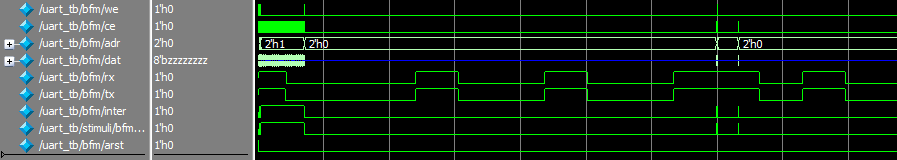
\includegraphics[ width= \textwidth]{rxIsTx.png}
	  \captionof{figure}{Mise en évidence de la relation entre le fil RX et TX}
	  \label{rxtx:rxtxscreenshot}
	\end{center}
	% Fin screenshot

        % Screenshot
	\begin{center}
	  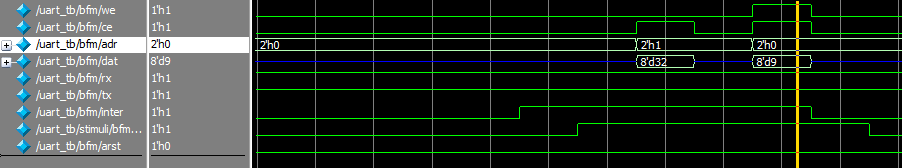
\includegraphics[ width= \textwidth]{write9.png}
          \captionof{figure}{\refToStep{rxtx:firststep}{Écriture de la valeur 9 par \udriver vers \theDut}}
	  \label{rxtx:firststepscreenshot}
	\end{center}
	% Fin screenshot

        % Screenshot
	\begin{center}
	  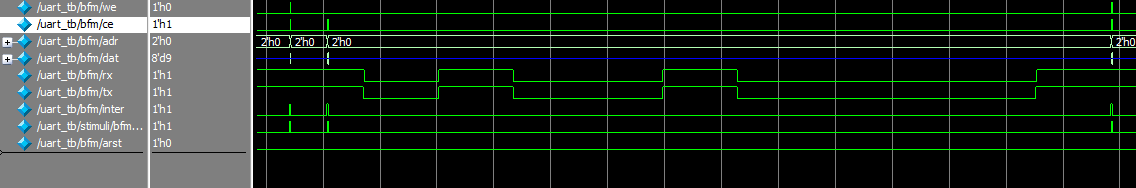
\includegraphics[ width= \textwidth]{serial9.png}
          \captionof{figure}{\refToStep{rxtx:secondstep}{Transmission sérielle par \theDut vers \udriver}}
	  \label{rxtx:secondscreenshot}
	\end{center}
	% Fin screenshot


        % Screenshot
	\begin{center}
	  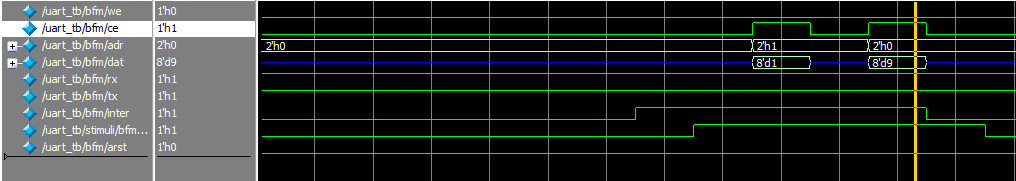
\includegraphics[ width= \textwidth]{read9.png}
	  \captionof{figure}{\refToStep{rxtx:thirdstep}{Lecture par \udriver de la valeur transmise sériellement}}
	  \label{rxtx:thirdstepscreenshot}
	\end{center}
	% Fin screenshot
\section{Modification du DUT pour plan de test}
    \subsection{Test de transmission}
        \lipsum[1]
    \subsection{Test de réception}
        \lipsum[1]

\section{Amélioration de la génération aléatoire} 
    \subsection{Création de la classe \uconfig} \lipsum[2]
    \subsection{Contenu de la classe \uconfig} \lipsum[2]
    \subsection{Modification de l'initialisation des modules} \lipsum[2]
    \subsection{Modification du programme de test} \lipsum[2]
    \subsection{Vérification du changement de parité} \lipsum[2]
    \subsection{Méchanisme de génération aléatoire} \lipsum[2]

\section{Injection d'erreurs} 
    \subsection{Injection du Parity Error} \lipsum[3]
    \subsection{Injection du Framing Error} \lipsum[3]
    \subsection{Injection du Data Error} \lipsum[3]

\section{Couverture}
    \subsection{Groupe de couverture} \lipsum[4]
    \subsection{Croisement} \lipsum[4]
    \subsection{Automatisation de la fin de test} \lipsum[4]

\section{Assertions}
    \subsection{Description et fonctionnement de TODO } \lipsum[5]
    \subsection{Description et fonctionnement de TODO } \lipsum[5]
    \subsection{Description et fonctionnement de TODO } \lipsum[5]
\end{document} 
